
%(BEGIN_QUESTION)
% Copyright 2010, Tony R. Kuphaldt, released under the Creative Commons Attribution License (v 1.0)
% This means you may do almost anything with this work of mine, so long as you give me proper credit

Contract personnel have wired and programmed this PLC/HMI system to control the opening and closing of a motor-operated valve (MOV).  However, a problem exists within the programming of this system despite the fact that the contractors have taken the money and fled.  Note that the electrical wiring is simplified in this illustration (e.g. no common terminals or wiring shown, no internal diagrams), and no color highlighting is shown in the PLC's program:

$$\includegraphics[width=15.5cm]{i02390x01.eps}$$

First, explain what is wrong with the programming, then edit the PLC program to fix the problem.

\underbar{file i02390}
%(END_QUESTION)





%(BEGIN_ANSWER)

{\it Award half-credit for properly identifying the problem, and half-credit for a complete fix.}

\vskip 10pt

The problem is that the HMI is trying to directly write to PLC bits Y1 and Y2, causing a conflict with the Y1 and Y2 coils in the PLC program.  The HMI and PLC programs should be re-written as such, with the HMI triggering ``C'' bits with contact instructions in parallel with the hard-wired X1 and X2 ``Start'' and ``Stop'' inputs.

$$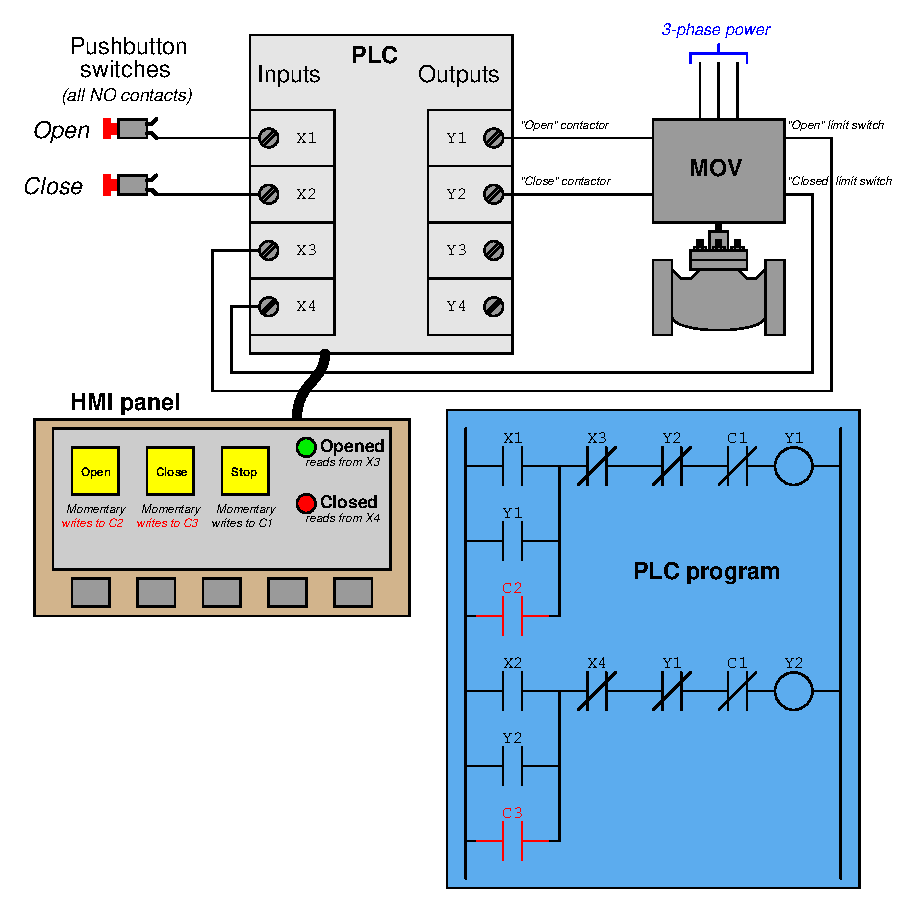
\includegraphics[width=15.5cm]{i02390x02.eps}$$

%(END_ANSWER)





%(BEGIN_NOTES)

{\bf This question is intended for exams only and not worksheets!}.

%(END_NOTES)

